\section{Modulatorer}
\index{modulatorer}

\subsection{Allmänt}
\index{modulation}

När en signal (bärvågen) påverkas så att den överför informationen i
en annan signal, sägs bärvågen bli modulerad. Detta förlopp kallas
modulation. Vad som då händer behandlas främst i avsnitt
\ref{modulation}, med tillämpningar i kapitel \ref{sändare} och delvis i
kapitel \ref{mottagare}.

En anordning för modulation kallas för modulator. En modulator kan
ingå som en funktion i sändare, mottagare m.fl. system.  Beroende på
modulationsmetoden används olika kombinationer av delkretsar som
tillsammans utgör modulatorn.

I detta avsnitt ges exempel på några vanliga modulatorer för sändare.

\subsection{Amplitudmodulatorer}
\index{amplitudmodulator}
\index{amplitudmodulation (AM)}

Med en amplitudmodulator påverkas bärvågens amplitud proportionellt
med den modulerande signalens amplitud.

\index{A1A}
\emph{Vid sändningsslaget A1A} är amplituden på den modulerande
signalen antingen maximal eller ingen. Då består modulatorn av en
nycklingskrets, som påverkar t.ex. ett drivsteg i sändaren så att
bärvågen släpps fram helt eller inte alls.

\index{A3E}
\emph{Vid sändningsslaget A3E} har den modulerande signalens amplitud
ett analogt förlopp, t.ex. tal, med vilket bärvågens amplitud
moduleras. Här beskrivs amplitudmodulation i en förstärkare med ett
katodkopplat elektronrör. En emitterkopplad transistorförstärkare kan
moduleras på ett liknande sätt. I båda fallen moduleras förstärkarens
arbetsspänning (anodspänning resp. kollektorspänning) med den
modulerande signalens. Det som då händer är att två signaler blandas
på ett sätt som beskrivs i avsnitt \ref{modulation} med tillämpning på A3E.
I vila är då bärvågsamplituden halva den möjliga inom arbetskurvans linjära
del. Vid modulation kommer bärvågens amplitud att variera mellan noll
och den möjliga amplituden.

\begin{wrapfigure}{R}{0.5\textwidth}
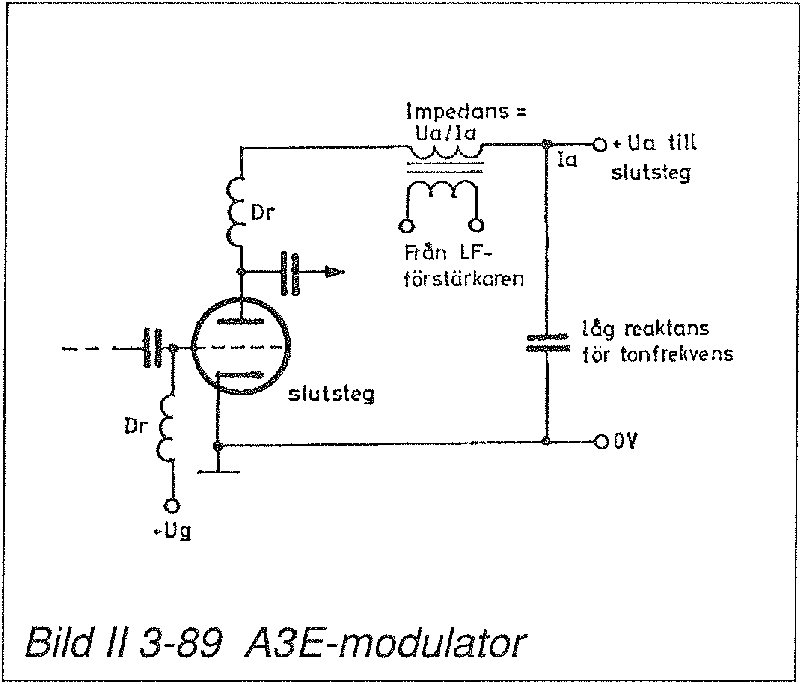
\includegraphics[width=0.5\textwidth]{images/bild_2_3-89}
\caption{A3E-modulator}
\label{fig:BildII3-89}
\end{wrapfigure}

Bild \ref{fig:BildII3-89}

Bilden visar ett sändarslutsteg med en triod.  I serie med
tilledningen för anodspänningen finns sekundärlindningen av en
modulationstransformator för LF-signalen.

Den LF-förstärkare som driver transformatorn måste för 100~\%
modulationsgrad kunna avge bärvågens halva effekt. Eftersom uteffekten
från en fullt utmodulerad A3E-sändare är 150~\% av den i vila, måste
slutsteget dimensioneras därefter. Utöver den egna signalspänningen
måste modulationstransformatorn även klara slutstegets arbetsspänning.

\index{klass A}
\index{klass C}
Om som på bilden anodspänningen i ett förstärkarsteg amplitudmoduleras,
kan förstärkarsteget arbeta olinjärt, t.ex i klass C.
Varje följande förstärkarsteg måste däremot arbeta linjärt, t.ex. i klass A.

På grund av den låga verkningsgraden och det stora bandbreddsbehovet,
används i dagens amatörradiosändare knappast ''äkta''
amplitudmodulering, d.v.s. A3E. I stället används i läget ''AM'' nästan
alltid H3E, d.v.s. enkelt sidband med full eller reducerad bärvåg (se
nästa stycke). Trots det lägre effektbehovet p.g.a. endast ett sidband
och ev. reducerad bärvågsamplitud kan av dimensioneringsskäl ändå inte
de flesta H3E-sändare avge sin fulla effekt kontinuerligt!

Som redan sagts i avsnitt \ref{modulation}, är det onödigt sända ut två sidband,
eftersom båda innehåller samma information. Det räcker med ett
sidband. Bärvågen innehåller inte någon information. Den kan därför
undertryckas redan i sändaren för att ersättas i mottagaren. Därmed
uppstår sändningsslaget J3E.

\subsection{Vid sändningsslaget J3E (SSB)}
\index{Single Side Band (SSB)}
\index{SSB}
\index{J3E}

Vid sändningsslaget J3E (SSB) sänds således endast ett sidband. Det
andra sidbandet och bärvågen undertrycks, vilket kan göras på flera
sätt. Numera är den s.k. filtermetoden allra vanligast och den enda
som behandlas här.

\begin{figure}
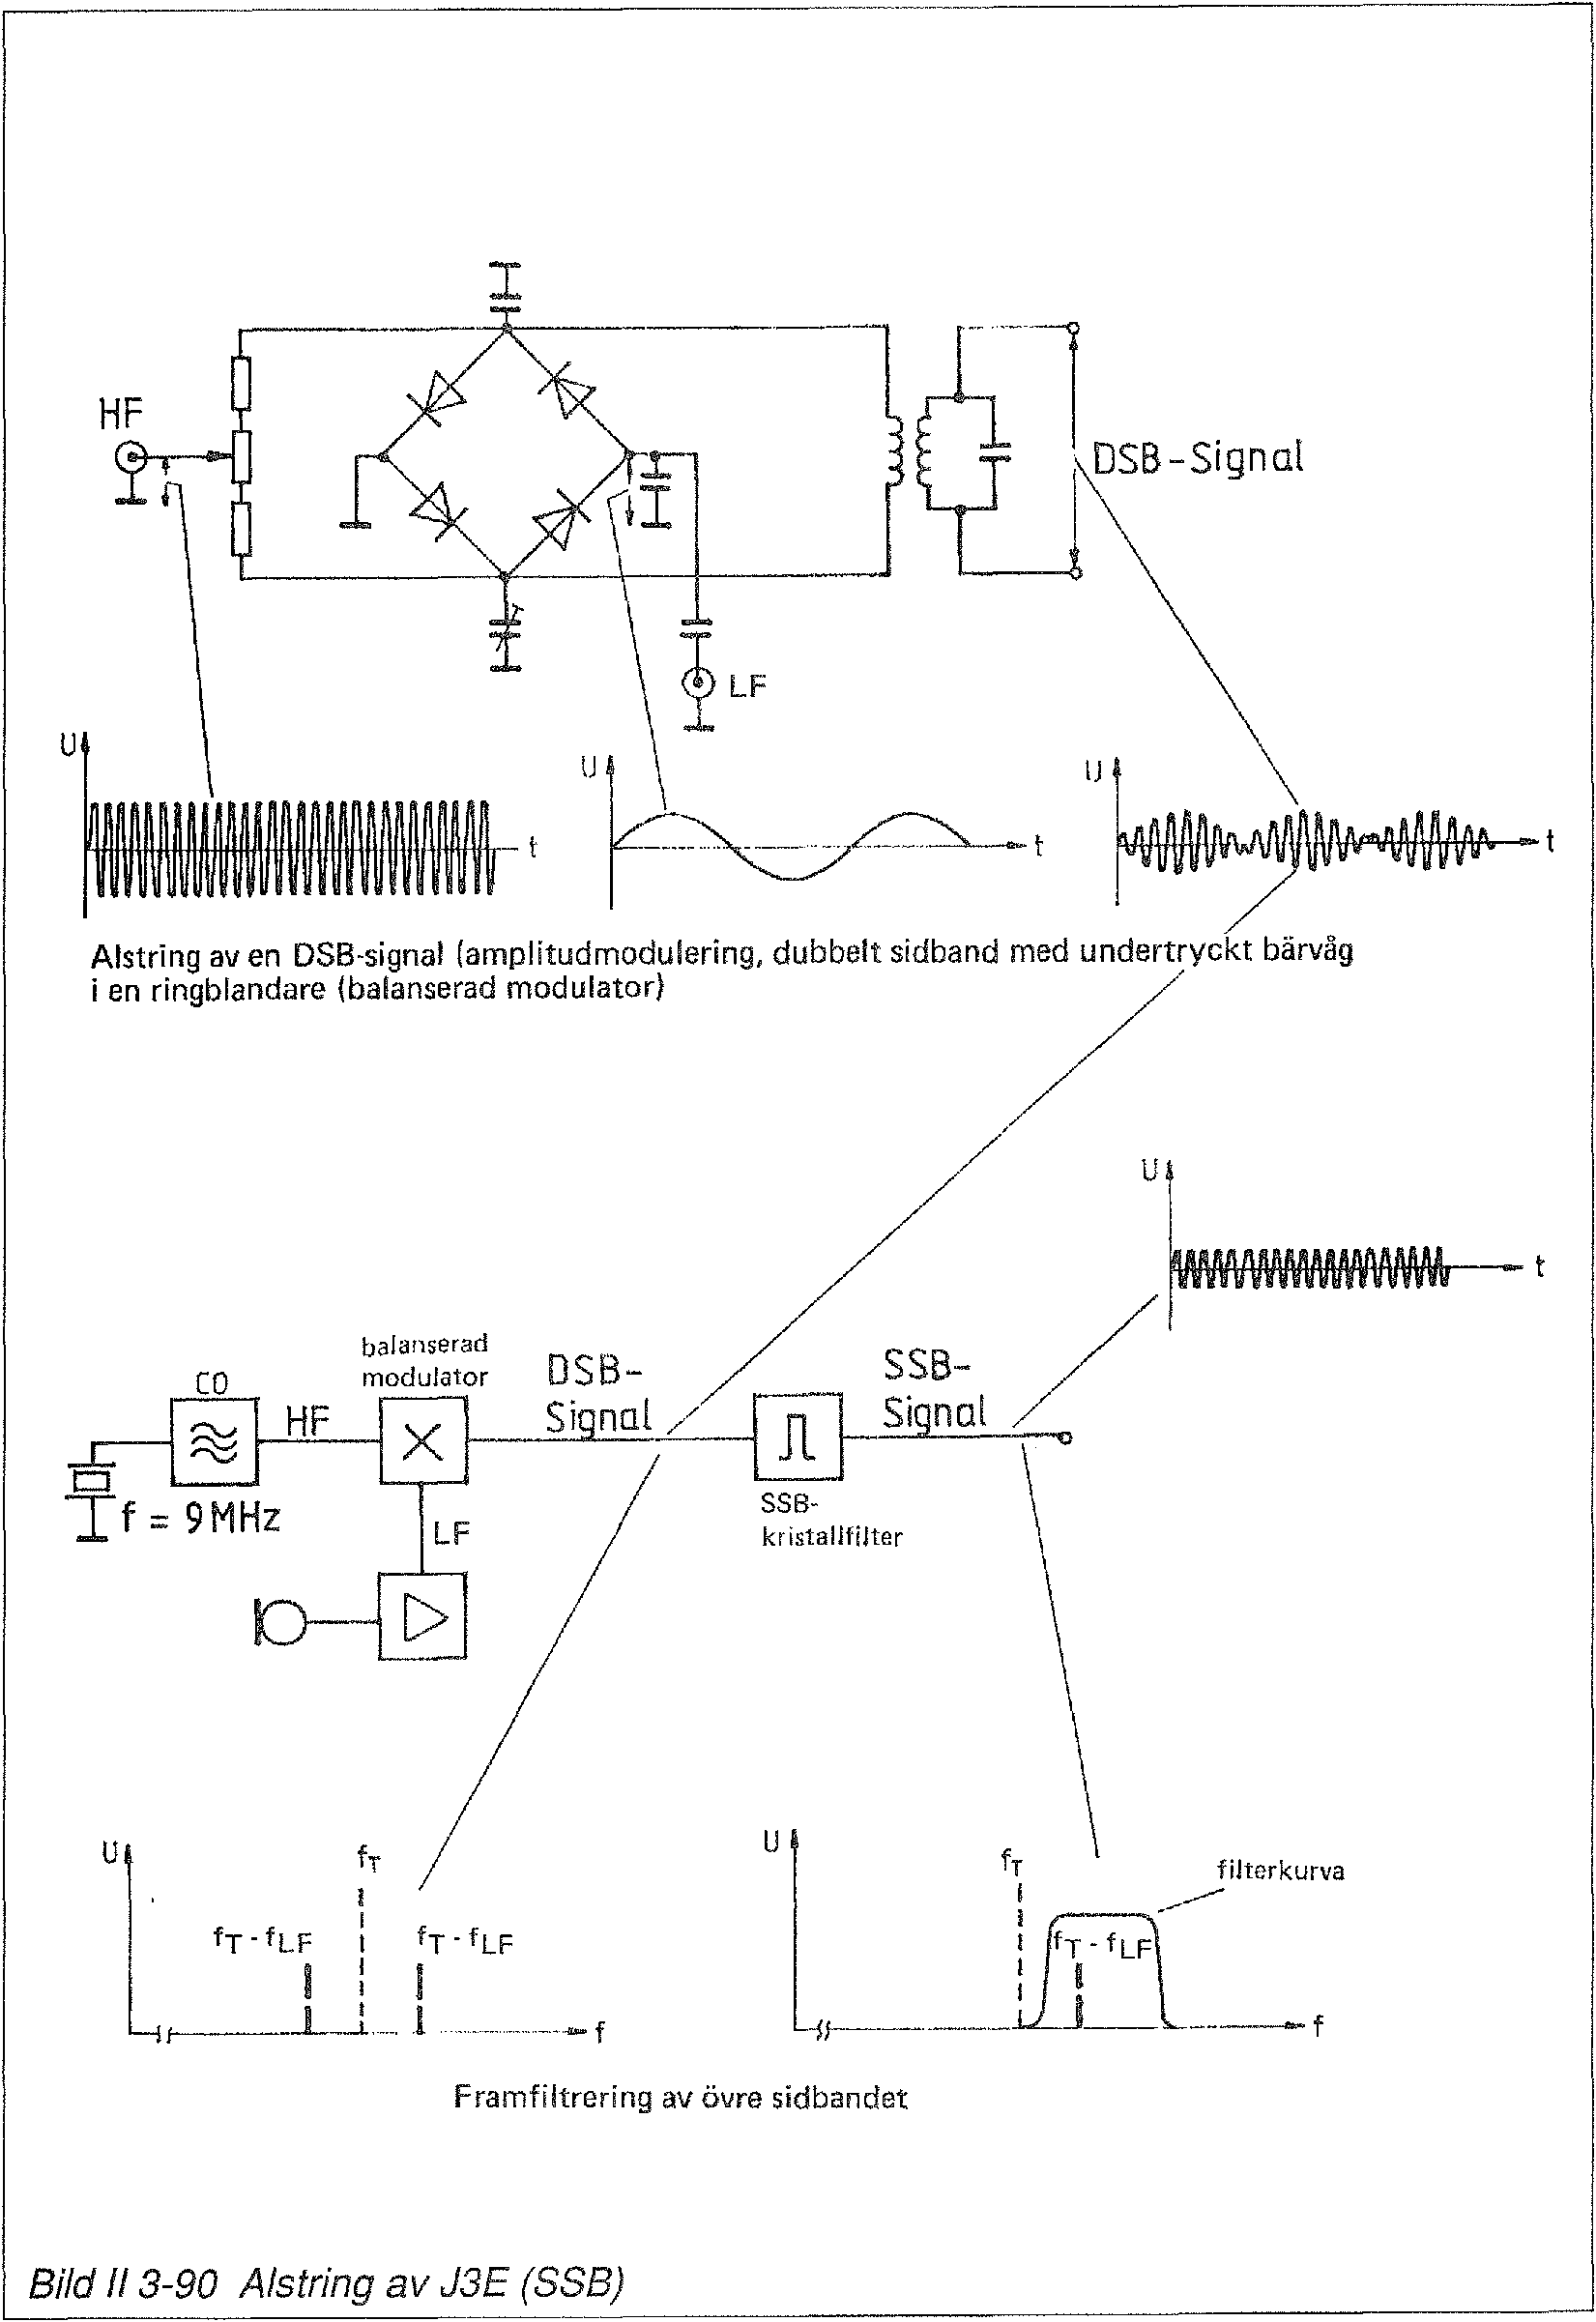
\includegraphics[width=\textwidth]{images/bild_2_3-90}
\caption{Alstring av J3E (SSB)}
\label{fig:BildII3-90}
\end{figure}

Bild \ref{fig:BildII3-90}

\index{Upper Side Band (USB)}
\index{USB}
\index{Lower Side Band (LSB)}
\index{LSB}

Med filtermetoden blandas HF- och LF-signalerna i en balanserad
blandare där de undertrycks medan blandningsprodukterna med deras
summa- och skillnadsfrekvenser blir kvar, d.v.s. det övre och nedre
sid bandet.

För att undertrycka det ena sidbandet före sändningen, följs blandaren
av ett bandpassfilter med bandbredd och frekvensläge för avsett
sidband. Den signal som sänds ut innehåller på så sätt endast ett
sidband (Single Side Band).

Valet mellan USB och LSB kan göras på två sätt. Antingen genom att
välja mellan ett separat passbandfilter för respektive sidband eller
genom att använda ett enda filter och flytta HF-signalen från ena
sidan till den andra av det filtret (se bild \ref{fig:BildII1-28} i
avsnitt \ref{modulation}).

En J3E-modulator enligt filtermetoden består således av en balanserad
blandare ofta en s.k. ringblandare (se bild \ref{fig:BildII3-87} i avsnitt
\ref{blandare}) samt ett bandpassfilter.  För att SSB-signalen ska få avsedd
sändarfrekvens kan ytterligare frekvensblandning behövas (se kapitel
\ref{sändare}).

\subsection{Vinkelmodulation}
\index{vinkelmodulation}

Vinkelmodulation är samlingsnamnet för frekvensmodulation (FM) och
fasmodulation (PM).

\subsection{Frekvensmodulation}
\index{frekvensmodulation (FM)}
\index{FM}
\index{F3E}

Vid sändningsslaget F3E (även kallat FM) varierar bärvågens frekvens i
takt med den modulerande signalens amplitud. Bärvågen kommer på så
sätt att pendla omkring en nominell frekvens, d.v.s. vara
frekvensmodulerad. Bärvågsamplituden ändras däremot inte vid
frekvensmodulation.

Likspänningsnivåer kan således överföras eftersom en frekvensavvikelse
(deviation) i bärvågen endast påverkas av den modulerande signalens
amplitud.

Vid F3E påverkas resonansfrekvensen i den svängningskrets i
oscillatorn som bestämmer dess arbetsfrekvens. Det görs enklast genom
att tillföra en kondensator med variabelt kapacitansvärde, en
s.k. varicap (se avsnitt \ref{varicap}).

\begin{figure}
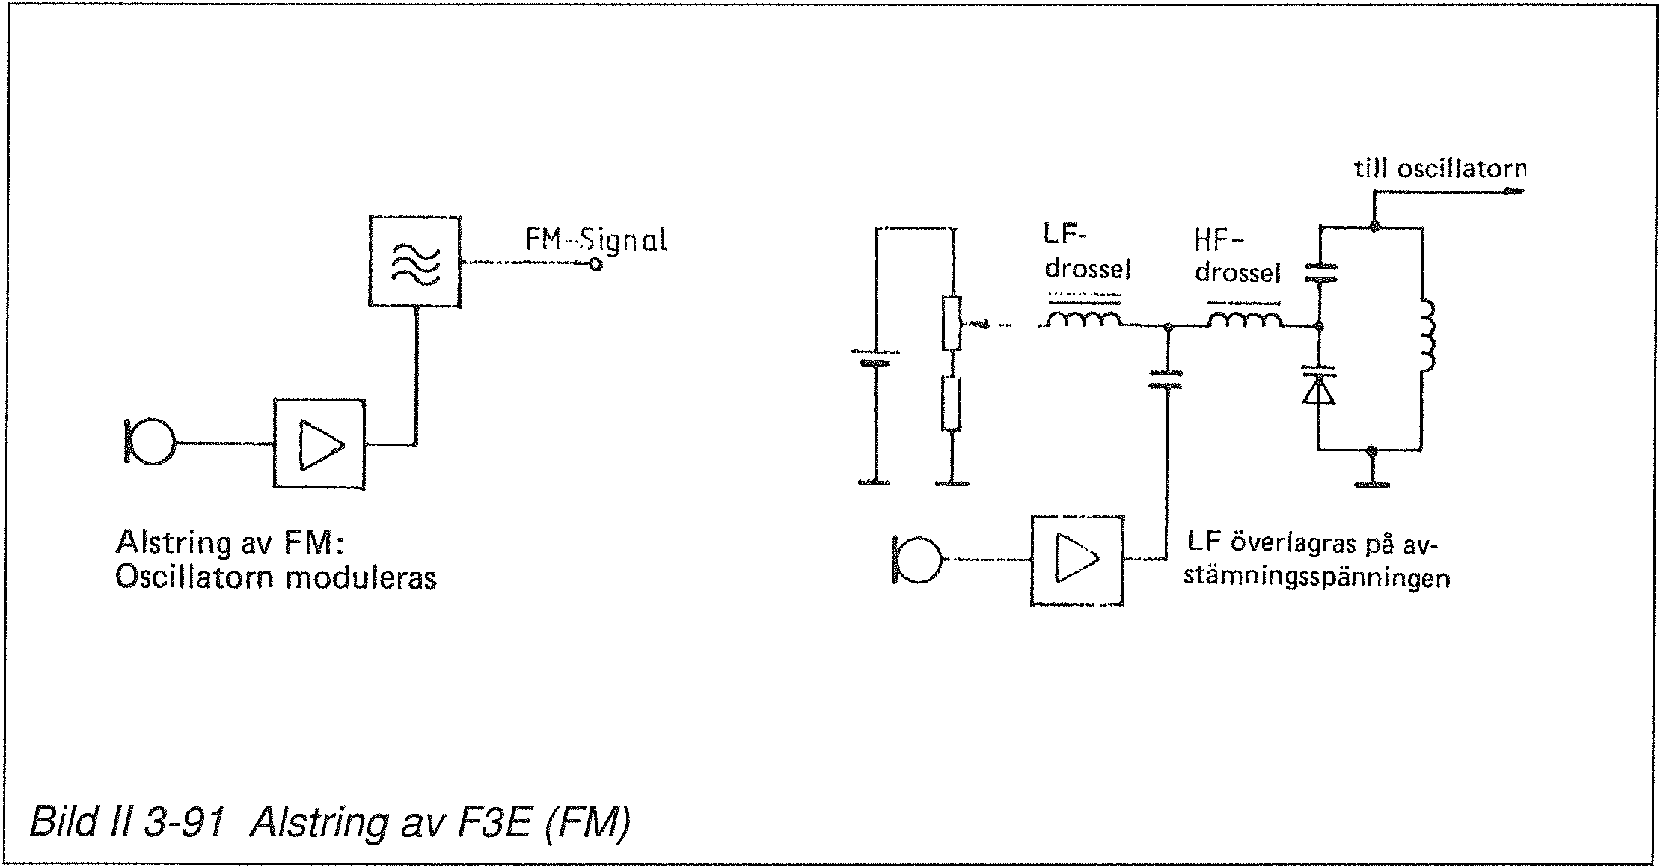
\includegraphics[width=\textwidth]{images/bild_2_3-91}
\caption{Alstring av F3E (FM)}
\label{fig:BildII3-91}
\end{figure}

Bild \ref{fig:BildII3-91}

Bilden visar en LC-svängningskrets där det ingår en varicapsom styrs
av en likspänning med en överlagrad modulerande LF-signal. En
likspänning tjänar som en ställbar förspänning till varicap. På så
sätt kan man påverka arbetsfrekvensen. Med den överlagrade LF-signalen
påverkas arbetsfrekvensen i takt med signalamplituden.

\subsection{Fasmodulation}
\index{fasmodulation}
\index{phasemodulation (PM)}
\index{PM}
\index{G3E}

Vid sändningsslaget G3E (även kallat PM) varierar bärvågens fasläge i
förhållande ,till en referens, som är en omodulerad bärvåg.  Bärvågens
amplitud ändras däremot inte. Fasändringen --- deviationen --- är direkt
proportionell till hur snabbt fasläget ändras och till den totala
fasändringen. Hastigheten på fasändringen är direkt proportionell till
frekvensen på den modulerande signalen och till dess amplitud.

Det betyder att deviationen vid fasmodulation ökar både med amplituden
och frekvensen på den modulerande signalen. Ändringar i
likspänningsnivåer kan därför överföras endast om en fasreferens
används.

Fasmodulation kan alstras t.ex. genom att påverka resonansfrekvensen i
en svängningskrets någonstans efter oscillatorn, d.v.s.  där
oscillatorfrekvensen inte påverkas. Denna svängningskrets har i
viloläge samma resonansfrekvens som oscillatorn. När kretsen bringas
ur resonans genom modulation --- samtidigt som kretsen påtrycks
oscillatorsignalen --- så uppstår i kretsen omväxlande en induktiv och
kapacitiv reaktans --- detta inom tiden för varje halv period. Reaktansen
skapar därvid den fasförskjutning som innebär fasmodulation. Se även
avsnitt \ref{parallellresonans} och \ref{serieresonans}, bilderna
\ref{fig:BildII3-18} och \ref{fig:BildII3-19}

\begin{figure}
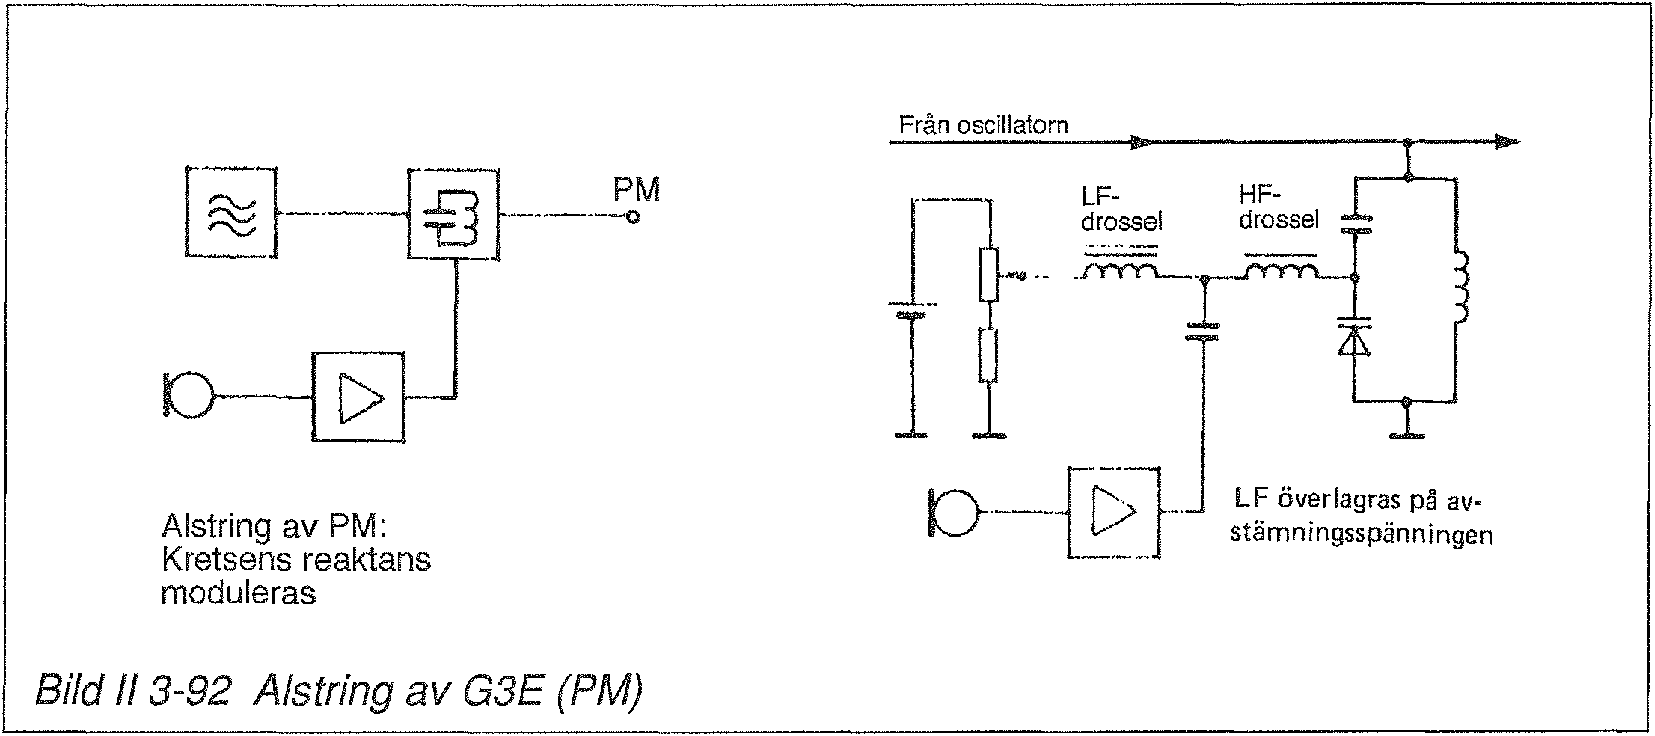
\includegraphics[width=\textwidth]{images/bild_2_3-92}
\caption{Alstring av G3E (PM)}
\label{fig:BildII3-92}
\end{figure}

Bild \ref{fig:BildII3-92}

Liksom vid frekvensmodulation kan t.ex. en varicap användas för att
med en modulerande signal påverka resonansfrekvensen i en krets.
